\section{Background and Related Work}
\label{sec:background}




% 介绍漏洞复现的定义、流程、难点
\subsection{Vulnerability Research}

\paragraph{Vulnerability Detection and Exploitation.}
%Automated vulnerability research is built on three intertwined lines.
Vulnerability discovery progressed from random robustness testing and static buffer-overrun checking to concolic, whitebox, coverage-guided, and hybrid fuzzing~\cite{fuzz,wagner2000first,godefroid2005dart,godefroid2008automated,bohme2016coverage,stephens2016driller,qsym}.
%Program analysis made these techniques applicable to complex binaries through symbolic execution, dynamic taint tracking, dynamic instrumentation, and reusable binary-analysis platforms~\cite{king1976symb,newsome2005taintcheck,nethercote2007valgrind,song2008bitblaze,s2e,angr}.
Exploitation research
%evolved from manual stack smashing and return-oriented programming
aims to automatic exploit generation and autonomous cyber-reasoning systems~\cite{alephone1996stack,shacham2007geometry,brumley2008patchaeg,avgerinos2014automatic,cha2012unleashing,shoshitaishvili2018mechanical}.
%These works establish how to find, analyze, and demonstrate the exploitability of a flaw once a program is available, whereas our setting additionally asks an agent to identify, acquire, build, and operationalize the affected target from only a CVE identifier.

\paragraph{IoT Vulnerability Detection.}
%For IoT devices, vulnerability reproduction is particularly challenging.
Existing IoT vulnerability detection efforts predominantly rely on static analysis~\cite{karonte,satc,emtaint,hermescan,mango,nvwa}, which can identify candidate vulnerability paths but cannot confirm their triggerability in a real runtime environment~\cite{challenges}. Transforming static analysis reports into verified results requires dynamic validation on the actual firmware binary, a process that is largely manual and demands expert knowledge of firmware rehosting~\cite{firmadyne,firmae,greenhouse,pandawan}. The core difficulty lies in rehosting: proprietary firmware images are tightly coupled to specific hardware and often cannot be stably launched in emulation environments~\cite{fuzzware,firmafl}.

\paragraph{Vulnerability Reproduction.}
Vulnerability reproduction is the process of demonstrating that a known vulnerability exists by producing a proof-of-concept (PoC) that triggers the bug~\cite{cybergym}. Recent work has explored automating this process with LLM agents\cite{liu2026cve2poc,zhao2025systematic, krepro}.
In practice, a security analyst reproduces a vulnerability starting from a CVE identifier by multi-steps and these activities have prerequisites, although agents can revisit earlier work or use alternative execution paths. An unmet prerequisite can prevent later real-target execution. This means that the full reproduction pipeline is far more demanding than the final triggering step alone.


\begin{figure}[t]
    \centering
    \begin{tikzpicture}[>=Latex,
 box/.style={draw,rounded corners,align=left,text width=2.85in,inner sep=5pt,font=\small}]
\node[box,fill=black!3] (prepared) {\textbf{Prepared-target setting}\\Source, binary, or running service supplied\\Agent analyzes and tests the supplied target};
\node[box,below=0.20in of prepared,fill=blue!4] (cve) {\textbf{Studied CVE-only setting}\\CVE identifier + common execution setup\\Agent identifies, acquires, prepares, and tests the target};
\end{tikzpicture}

    \caption{Task starting conditions. Prepared-target settings supply an executable target; the studied CVE-only setting also requires acquisition and preparation. These are task settings, not an exhaustive division of prior work.}
    \label{fig:iceberg}
\end{figure}

% 网络安全benchmark，按四类漏洞任务分组
\subsection{Cybersecurity Benchmarks}
% Existing cybersecurity benchmarks can be grouped by which stage of the vulnerability lifecycle they evaluate: \emph{discovery} (finding an unknown vulnerability), \emph{reproduction} (producing a PoC that triggers a known vulnerability), \emph{exploitation} (escalating a bug into a concrete security impact), and \emph{patching} (generating a code fix).
% For discovery, they usually provide the source code for
% the target programs (\cite{cybergym, cvebench, cybergyme2e, bountybench}).
% For reproduction, beside the target program, they also need some more things, e.g., vulnerability description, a PoC script or a patch file (\cite{krepro, secbench}).
% For exploitation and patching, they usually need a execution binary, a containerized or a running service before they conduct the evaluation (\cite{exploitbench, exploitgym, cybergyme2e}).
Existing cybersecurity benchmarks evaluate diverse security tasks---vulnerability discovery, reproduction, exploitation, and patching---but they differ most in what target access they assume at the start.
Some hand the agent source code or a project repository~\cite{cybergym,secbench,cvebench,bountybench}; others provide patch context, vulnerability descriptions, or reference PoCs~\cite{krepro,secbench}; and still others start from a built binary, a container, or a running service~\cite{exploitbench,exploitgym,cybergyme2e}.
These settings allocate different parts of target preparation to the benchmark and the agent. CVE-GENIE explicitly reconstructs environments~\cite{cvegenie}; our study examines general coding agents navigating the combined IoT firmware workflow.

\subsection{From-Scratch Reproduction Gap}
Figure~\ref{fig:iceberg} highlights the starting condition studied here: the agent receives a CVE identifier and must identify, acquire, and prepare the affected firmware target. We use the pre/post-environment distinction to describe task conditions, without claiming that all prior work omits environment construction. The six-phase analysis records progress and recurring failures within this combined workflow.

Empirical reproduction studies similarly connect outcomes to information availability and troubleshooting~\cite{mu2018crowdrepro}. The Web PoC study combines a curated vulnerability benchmark with research-question-driven experiments~\cite{zhao2025systematic}. Here, the case collection and scoring rubric support the empirical analysis rather than define the knowledge contribution by themselves.

\begin{figure*}[t]
    \centering
    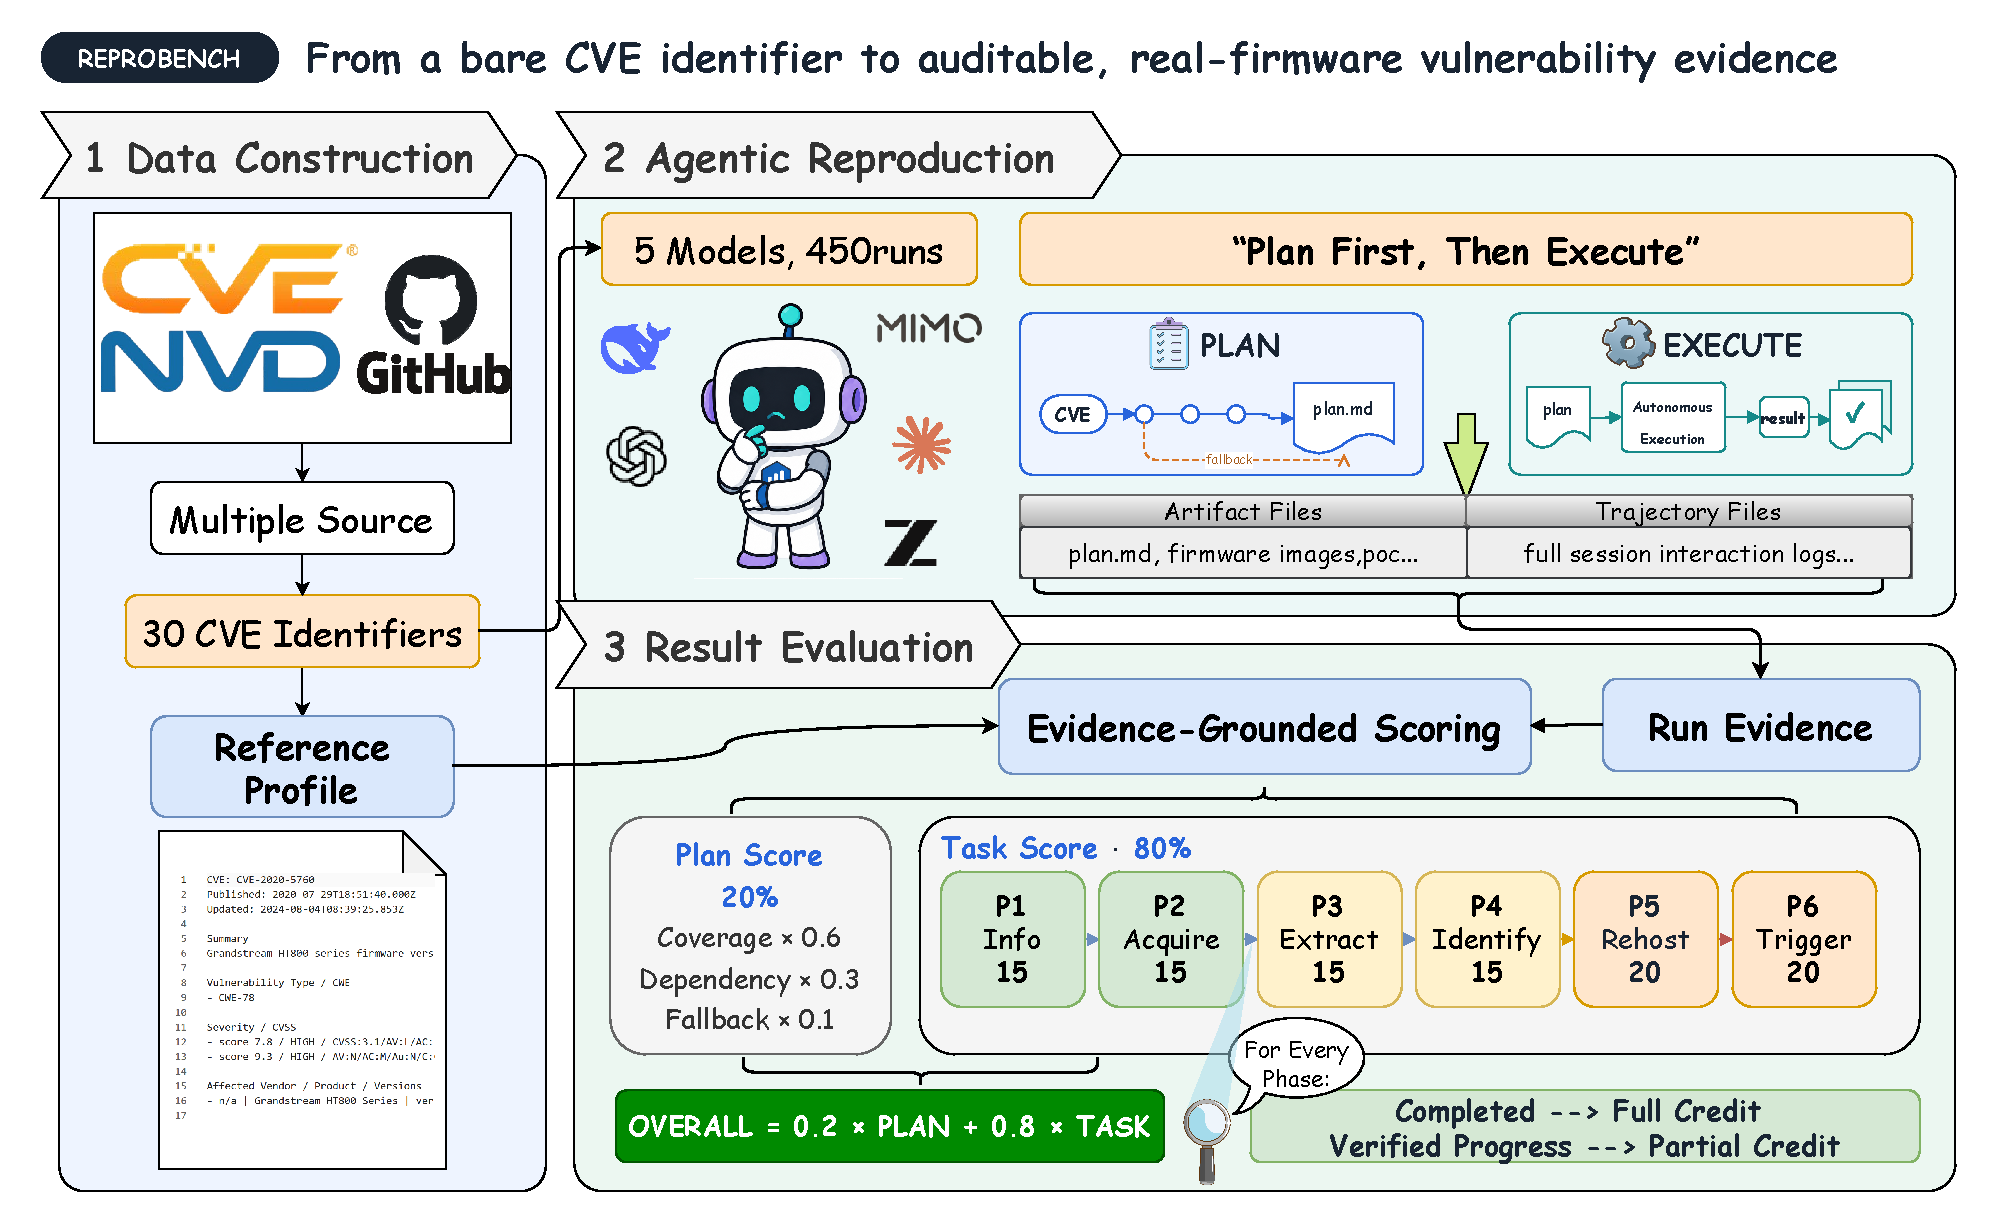
\includegraphics[width=\textwidth]{figures/framework0724.pdf}
    \caption{Study workflow, retaining the original six-phase scoring organization. CVEs are curated and paired with public evidence. Agents receive only a CVE identifier and must plan, execute, and report. The scoring skill evaluates each run against the public evidence.}
    \label{fig:framework}
\end{figure*}
